158. \begin{figure}[ht!]
\center{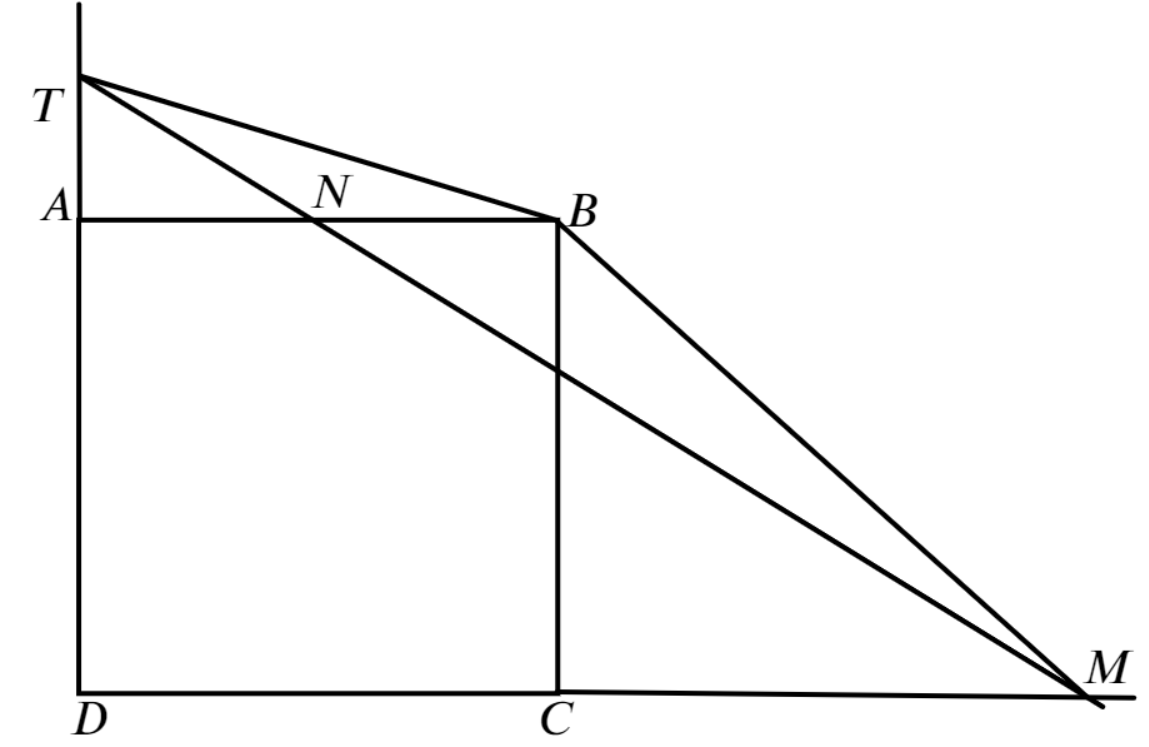
\includegraphics[scale=0.35]{g9-158.png}}
\end{figure}\\
$tg(\angle NTA)=\cfrac{NA}{TA}=2,$ значит $TA=3:2=\cfrac{3}{2}.$ Тогда $S_{\Delta BMT}=S_{\Delta BMN}+S_{\Delta BTN}=\cfrac{1}{2}\cdot6\cdot3+\cfrac{1}{2}\cdot\cfrac{3}{2}\cdot3=\cfrac{45}{4}$ (площади посчитаны через высоты, опущенные из точек $M$ и $T$).\\
